\documentclass[usenames,dvipsnames]{beamer}
%\documentclass[handout]{beamer}

% language settings
%\usepackage{fontspec, polyglossia}
%\setdefaultlanguage{magyar}

% common packages
\usepackage{amsmath, multimedia, hyperref, color, multirow}
%\usepackage{graphicx}

% TikZ
\usepackage{tikz}
%\usetikzlibrary{arrows.meta, decorations.pathmorphing, decorations.pathreplacing, shapes.geometric,mindmap}
%\usetikzlibrary{shapes.geometric,fadings,bayesnet}

% beamer styles
\mode<presentation>{
%\usetheme{Warsaw}
%\usetheme{Antibes}
\usecolortheme{beaver}
%\usecolortheme{seahorse}
%\usefonttheme{structureitalicserif}
\setbeamercovered{transparent}
}
\setbeamertemplate{blocks}[rounded][shadow=true]
\AtBeginSubsection[]{
  \begin{frame}<beamer>{Contents}
    \tableofcontents[currentsection,currentsubsection]
  \end{frame}
}
%\useoutertheme[]{tree}

% title, etc
\title{The Main Title Naming Key Concepts}
\subtitle{A subtitle may be shorter and more technical}
\author{Attila Jones}
\date{}

\begin{document}

\begin{frame}{Network proximity}{Cheng et al 2018 Nat Commun}
\includegraphics[width=1.0\textwidth]{../figures/from-others/cheng-desai-2018-Nat-comm-SFig1b.png}
\begin{description}
\item[$T$] target gene set 
\item[$t$] some target gene 
\item[$S$] disease gene set 
\item[$s$] some disease gene 
\end{description}
\[
d(S, T) = \frac{1}{|T|}\sum_{t \in T} \min_{s \in S} d(s, t)
\]
\end{frame}

\begin{frame}{Proximity and its statistical significance}
\begin{columns}[t]
\begin{column}{0.45\textwidth}

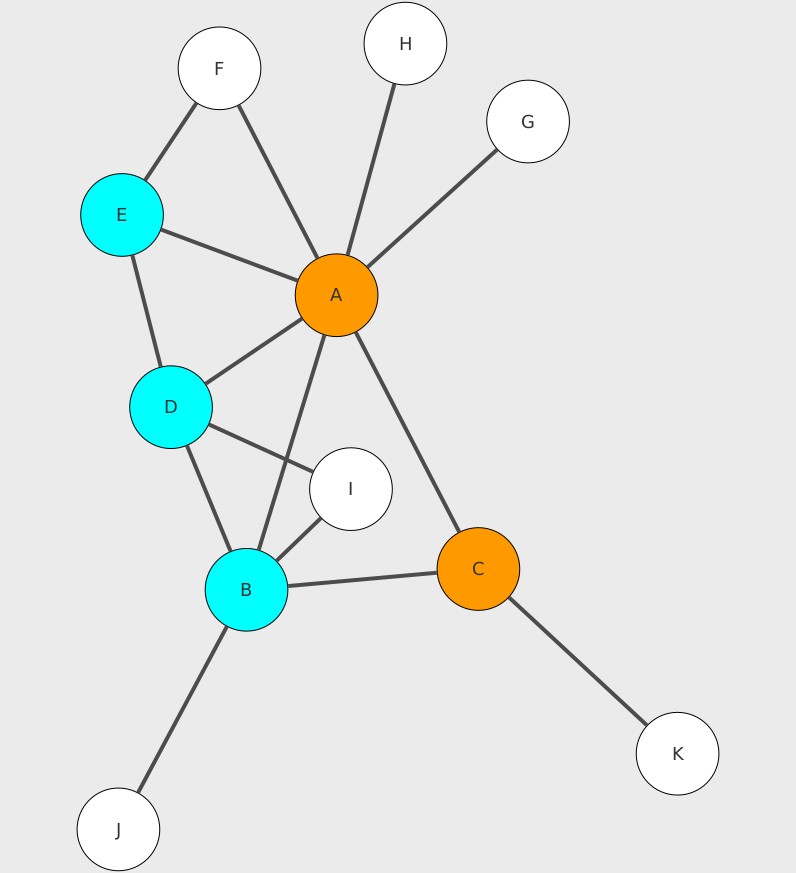
\includegraphics[width=\columnwidth]{../figures/toy.sif.png}
\end{column}

\begin{column}{0.55\textwidth}
Proximity
\small
\begin{eqnarray*}
\textcolor{Orange}{\text{target genes} \; T} &=& \{A, C\} \\
\textcolor{Cyan}{\text{disease genes} \; S} &=& \{B, D, E\} \\
\text{proximity} \; d(\textcolor{Orange}{S}, \textcolor{Cyan}{T}) &=& \frac{1}{4} \overbrace{(1 + 1 + 1 + 1)}^{\text{shortest path lengths}} \\
&=& 1 \\
\end{eqnarray*}
\normalsize
Significance

\small
$d(S', T') \sim \mathcal{N}(\hat{\mu}_0, \hat{\sigma}_0)$ null dist.

$\{S': S' \cong \textcolor{Orange}{S}\}$ and $\{T': T' \cong \textcolor{Cyan}{T}\}$
\begin{eqnarray*}
Z &=& \frac{d(\textcolor{Orange}{S}, \textcolor{Cyan}{T}) - \hat{\mu}_0}{\hat{\sigma}_0} = \frac{1 - 0.687}{0.242} = 1.294 \\
p &=& 0.902 \; \text{ for } \; \mathcal{H}_0: \mu_{S,T} < \mu_0
\end{eqnarray*}
\end{column}
\end{columns}
\end{frame}

\begin{frame}
\includegraphics[height=0.9\textheight]{../figures/by-me/network-repos-flowchart/network-repos-flowchart.pdf}
\end{frame}

\begin{frame}{AD candidate gene prioritization with Endeavour}
\includegraphics[width=1.0\textwidth]{../figures/from-others/endeavour-2016-Fig1.jpg}

\tiny{Tranchevent et al 2016 Nucleic Acids Res}
\end{frame}

\end{document}

\begin{columns}[t]
\begin{column}{0.5\textwidth}

\end{column}

\begin{column}{0.5\textwidth}

\end{column}
\end{columns}
